\chapter{Теоретическое обоснование}

Эта глава будет посвещена теоретическому исследованию вопроса нетранзитивности. Будет произведен расчет необходимых вероятностей и исследование силы нетранзитивности полученных соотношений.

\section{Причина отсутствия транзитивности}

Приведем обоснование при $a = 0.6\%$, $b = 0.3\%$, $c = 0.3\%$, $d = 0.6\%$. Здесь $a, b, c, d$ аналогичны тем, что были введены в предыдущей главе.
\smallskip
\smallskip

Вероятность того, что при работе с одними и теми же акциями на одном и том же временном интервале вторая стратегия приведет к реализации бумаг по более высокой цене, чем первая, равна приблизительно $2 \over 3$ или $66.7\%$. Это следует из того, что ожидаемая вероятность изменения на $0.6\%$ должна быть в два раза меньше, чем на $0.3\%$. Таким образом, вторая стратегия в указанном смысле оказывается лучше первой, то есть доминирует над ней. 
\smallskip
\smallskip

С другой стороны, вероятность того, что при аналогичных условиях третья стратегия позволит продать бумаги дороже, в сравнении со второй, также превышает $50\%$. Это следует из того, что на росте акции мы с большей вероятностью зафиксируем большую прибыль, а на падении меньший убыток. То есть третья стратегия, в свою очередь, доминирует над второй.
\smallskip
\smallskip

Предполагая транзитивность определенного нами отношения доминирования, можно подумать, что третья стратегия является самой предпочтительной из всех трех. Однако эта гипотеза не будет соответствовать действительности, так как на самом деле первая стратегия обеспечивает более высокую цену продажи по сравнению с третьей опять же с вероятностью примерно $66.7\%$. Далее мы подтвердим это строго.

\section{Расчет вероятностей}

Введем случайные величины, соответствующие прибыли для каждой из трёх стратегий. Введем их для удобства вычислений следующим образом:

\begin{center}
$X_1 \equiv 0$, 
$X_2$ = 
 \begin{cases}
   -a, &\text{с вер. $p_{-}(a, b)$}\\
   $\hspace{10pt}$ b, &\text{с вер. $p_{+}(a, b)$}
 \end{cases},
$X_3$ = 
 \begin{cases}
   -c, &\text{с вер. $p_{-}(c, d)$}\\
   $\hspace{9pt}$d, &\text{с вер. $p_{+}(c, d)$}
 \end{cases}
\smallskip
\end{center}


Тогда будет верно, что $P(X_1 < X_2) = p_{+}(a,b)$, $P(X_2 < X_1) = p_{-}(a,b)$. Аналогично $P(X_1 < X_3) = p_{+}(c,d)$, $P(X_3 < X_1) = p_{-}(c,d)$. Вычислим $p_{+}(a,b), p_{-}(a,b)$, вероятности $p_{+}(c,d), p_{-}(c,d)$ будут после этого определены автоматически.
\smallskip
\smallskip

Пусть $S_0$ - это стоимость акции в начале торгового дня. Пусть $A = {a\over{100\%}}$, $B = {b\over{100\%}}$, $p_{+}(a,b):= p_{+}$, $p_{-}(a,b):= p_{-}$. 
\smallskip
\smallskip

Будем использовать теорему Дуба об остановке$^{[2]}$. Тогда имеем, что:

\begin{center}
$S_0 = p_{+}S_0(1+B) + p_{-}S_0(1-A)$

$1 = p_{+}(1+B) + (1-p_{+})(1-A)$

$p_{+} = {A\over{A + B}} = {a\over{a + b}}, p_{-} = {b\over{a + b}}$
\end{center}

Тогда в примере, который мы описывали в предыдущей главе, будем иметь, что $p_{+}(0.6, 0.3) = {2\over{3}}, p_{-}(0.6, 0.3) = {1\over{3}}$.
\smallskip
\smallskip

Итого имеем, что:
\begin{center}
$p_{+}(a,b) = {a\over{a + b}}, p_{-}(a,b) = {b\over{a + b}}, p_{+}(c,d) = {c\over{c + d}}, p_{-}(c,d) = {d\over{c + d}}$
\end{center}


Теперь приступим к нахождению $P(X_2 < X_3)$. Сразу отметим, что случайные величины $X_2$ и $X_3$ зависимы, поэтому заполним таблицу вероятностей изменения цены акций ниже (не теряя общности будем считать, что $c < a$, $b < d$):

\begin{center}
   \begin{tabular}{|l|c|c|}\hline
    \diagbox[width=4em]{X_3}{X_2}&
      $-a$ & $b$ \\ \hline
      $-c$ & $p_{--}$ & $p_{+-}$ \\ \hline
      $d$ & $p_{-+}$ & $p_{++}$\\ \hline
    \end{tabular} 
\end{center}

Тогда будет верно, что $P(X_2 < X_3) = p_{--} + p_{-+} + p_{++}$. 
\smallskip
\smallskip

Верно, что $p_{--} = p_{-}(a, b) = {b\over{a + b}}$. Расчитывая вероятность таким образом, мы уверены, что цена акции не выйдет за полосу равную $b$ (а значит и $d$) и автоматически пересечет полосу $-c$.
\smallskip
\smallskip

Далее рассмотрим $p_{-+}$. Эта вероятность равна нулю, так как если $X_2 = -a$, то $X_3 = -c$, так как $c < a$. С другой стороны, если $X_3 = d$, то $X_2 = b$, так как $b < d$.
\smallskip
\smallskip

Наконец рассмотрим $p_{++}$. Аналогично рассуждению для $p_{--}$ будем иметь, что $p_{++} = p_{+}(c, d) = {c\over{c + d}}$. Имеем следующее: 


\begin{center}
    $P(X_2 < X_3) =  {b\over{a + b}} + {c\over{c + d}}$
\end{center}

Тогда получаем, что условие нетранзитивности можно записать в следующем виде:


\begin{center}
    $P(X_1 < X_2) > {1\over 2}, P(X_2 < X_3) > {1\over 2}, P(X_3 < X_1) > {1\over 2}$
    
    ${a\over{a + b}} > {1\over 2}, {b\over{a + b}} + {c\over{c + d}} > {1\over 2}, {d\over{c + d}} > {1\over 2}$
\end{center}

Еще раз проверим условие нетранзитивности для $a = 0.6$, $b = 0.3$, $c = 0.3$, $d = 0.6$.

\begin{center}
    ${a\over{a + b}} = {2\over 3} > {1\over 2}, {b\over{a + b}} + {c\over{c + d}} = {2\over{3}} > {1\over{2}}, {d\over{c + d}} = {2\over 3} > {1\over 2}$
\end{center}

Нетранзитивность доказана. Уделим внимание еще одному моменту. Докажем, что сумма вероятностей в таблице будет равна $1$. Для этого сначала вычислим  $p_{+-}$.
\smallskip
\smallskip

Необходимо рассмотреть два случая. Первый: стоимость сначала опускается до $-c$, а потом поднимается до $b$. Второй: стоимость сначала поднимается на $b$, а потом опускается на $-c$. Первая вероятность может быть вычислена так:  ${b\over{b + c}} * {a-c\over{a + b}}$. Вторая вероятность вычисляется так: ${c\over{b + c}} * {d-b\over{d + c}}$. Итого получаем, что $p_{+-} = {b(a-c)\over{(a + b)(b + c)}} + {c(d-b)\over{(b + c)(d + c)}}$. Перейдем к проверке:

\begin{center}
    $p_{--} + p_{-+} + p_{+-} + p_{++} = {b\over{a + b}} + {b(a-c)\over{(a + b)(b + c)}} + {c(d-b)\over{(b + c)(d + c)}} + {c\over{c + d}} = $
    
    ${b(b+a)\over{(a + b)(b+c)}} + {c(d+c)\over{(b + c)(c+d)}} = {b\over{b + c}} + {c\over{b + c}} = 1$
\end{center}
Равенство суммы вероятностей единицы выполнено. Теперь перейдем к решению оптимизационной задачи.

\section{Решение оптимизационной задачи}

Перейдем к исследованию полученных соотношений. Будем максимизировать силу нетранзитивности, а именно: 

\begin{center}
$min((P(X_1 < X_2), P(X_2 < X_3), P(X_3 < X_1)) \to max$

$min({a\over{a + b}}, {b\over{a + b}} + {c\over{c + d}}, {d\over{c + d}}) \to max$

$x := {a\over{a + b}}, y:= {d\over{c + d}}, 0 < x < 1, 0 < y < 1$

$min(x, 2 - x - y, y) \to max$

\end{center}

Минимум левого вырежния можно рассмотреть, как минимум из трех функций $f_1(x, y) = x, f_2(x,y) = 2 - x - y, f_3(x, y) = y$. Построим графики этих функций в одной системе координат и оставим их части соответствующие $min(f_1, f_2, f_3)$:

\begin{center}
    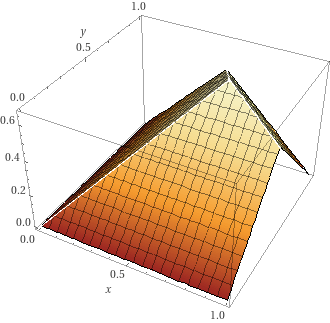
\includegraphics[keepaspectratio=true,scale=1]{images/chapter1/1.png}
\end{center}


Из графика видно, что максимум достигается в точке пересечения трех плоскостей, значит, надо приравнять все три функции, то есть $x = 2 - x - y = y$. Отсюда получаем что $x = y = {2 \over 3}$. Таким образом $({2 \over 3}, {2 \over 3})$  - точка максимума. 
\smallskip
\smallskip

Возвращаясь к изначальным переменным имеем, что сила нетранзитивности максимальна при $a = 2b$, $d = 2c$ сила нетранзитивности будет максимальной. Теперь перейдем к практической части.
